\section{Software}
As there exists a vast range of solutions for creating grids to represent real domains, learning, using and discussing all of them are way beyond the scope of this thesis. I will instead focus on two tools - MRST in \autoref{sec:MRST} and Gmsh in \autoref{sec:Gmsh}, as well as ways to combine the two tools in \autoref{sec:combining}. 

\subsection{MRST}
\label{sec:MRST}
The MATLAB Reservoir Simulation Toolbox - MRST - is an open-source toolbox for reservoir simulation, developed by the computational geosciences group at SINTEF Digital. Originally aimed at the study of discretization and flow solvers, the project has since expanded, and currently offers much of the same functionality that can be found in commercial reservoir simulators \cite{MRST_book}. Its main target is still research, with the primary focus being on rapidly developing and demonstrating contemporary methods and concepts \cite{MRST_website}.

In order to keep its extensive set of features maintainable, MRST is organized with a set of core functionality, as well as several optional add-on modules \cite{MRST_book}. The core includes methods for handling grids, data and basic mechanisms such as gravity, sources and wells, as well as an implementation of automatic differentiation. The add-on modules includes tools for discretization, solvers for incompressible flow, simulators based on automatic differentiation, specialized computational methods aimed at solving concrete problems, several utility modules, as well as tools that can be used to aid the modeling of the reservoirs. The latter group contains the UPR module.


\subsubsection{The UPR Module}
\label{sec:UPR}
Unstructured PEBI-grids for Reservoirs - UPR - was developed by \textcite{UPR_thesis}, as part of his 2016 Master thesis. The module is designed to generate PEBI grids conforming to well and faults, and can handle several challenging cases, such as multiple faults intersecting, intersections at sharp angles and intersections between wells and faults. The module also contain methods to generate such grids in three dimensions, but I will focus on 2D applications.

% Explain/show how UPR calculates well and fault sites
% Show examples
\paragraph{Well sites}
\label{UPR:wells}
UPR represents wells as cell centroids, and handles the base case, where the well follows a single line, by simply placing a set of well sites along the line. The distance between two sites along a line is not necessarily constant along the line, but care is taken such that the distribution satisfies the \emph{well condition} \cite[pp.42]{UPR_thesis}.

\begin{definition}[Well condition]
Let $p_1$ and $p_2$ be two consecutive well sites. The \emph{well condition} is satisfied if there exists a circle intersecting both points $p_1$ and $p_2$ that does not contain any other sites.
\end{definition}

It follows from Definition \ref{def:delaunay} that the edge between two consecutive well sites makes up an edge in a Delaunay triangulation if the well condition is satisfied, ensuring the two wells are neighbors in the PEBI grid. To simplify calculations, UPR uses a circle centered on the midpoint between two consecutive well sites to check the well condition \cite{UPR_thesis}.

Extra care is also taken when two wells intersect, as handling each well independently may lead to consecutive sites not connecting, or low-quality cells. To handle this, the intersecting wells are split and a well site is placed at the intersection. This well site is then shared among all intersecting at the point, i.e. all sites that now start or end at the intersection. 
% TODO: Example plot

UPR also allows protection sites around the well sites, in order to ensure regular well shapes and set a radius for the well. This is done by creating a pair of protection cells for each well site. These protection cells are placed normal to the well path, one on each side of the well site, with a distance equal to the target well radius. No protection sites are used for well intersection sites.
% TODO: Example plot

\paragraph{Fault sites}
\label{UPR:faults}
Faults are represented by cell edges, and are created by tracing the faults with two lines of fault sites - one on each side of the fault lines. UPR does this by creating a set of circles along the faults, then creating fault sites where these circles intersect. It first starts by placing a set of points, $C = \{c_i\}$ along the fault, with a distance between points given by a density function $d_i = \rho(c_i, c_{i+1})$. In order to create two fault points, two consecutive circles must intersect in two places. This creates the following distance limitations:
\begin{align}
    d_i &\le R_i + R_{i+1}  \label{eq:fault_distance_le}\\
    d_i &\ge \abs{R_i - R_{i+1}  \label{eq:fault_distance_ge}}
\end{align}
where $R_i$ is the radius of the circle centered at $c_i$. In UPR, the radius of each circle is set as the average of the distance to the circles on either side \cite{UPR_thesis}, i.e.
\begin{equation}
    R_i = c_f \frac{d_i + d_{i-1}}{2},
\end{equation}
where $c_f$ is a constant circle factor, determining the distance between the fault and the fault sites. Fault sites are then placed where two circles intersect, satisfying the \emph{fault condition}.
% TODO: Example plot

\begin{definition}[Fault condition]
Let $p_1$ and $p_2$ be two fault sites, placed at the intersection of the same pair of fault circles. The \emph{fault condition} is satisfied if the interior of the two fault circles does not contain any sites.
\end{definition}

The fault condition is enough to prove that the fault is traced by a face in the PEBI grid. Let $c_1$ and $c_2$ be the circles creating $p_1$ and $p_2$, and let $c_p$ be a point on the open line segment between $c_1$ and $c_2$. Let $c$ be a closed circle intersecting $p_1$ and $p_2$ with centroid $c_p$. $c$ is then an element in a subset of $\{c_1, c_2\}$, thus containing no other sites than $p_1$ and $p_2$. As $c$ intersects both $p_1$ and $p_2$, we have that
\begin{equation*}
    \abs{c_p - p_1} = \abs{c_p - p_2} < \abs{c_p - p}
\end{equation*}
for all other sites $p$. From Definition \ref{eq:voronoi-face}, $c_p$ must therefore be on the PEBI face $v_{p_1, p_2}$.
% TODO: Example plot

As with wells, extra care must be taken when fault lines intersect, as fault sites from different faults may disrupt the fault conditions. To handle these cases, faults are first split up at intersections, such that they may only appear at the start or end of each fault line segment. A fault circle is then placed at the intersection, and is shared by all fault lines starting or ending at the intersection. All other circles are placed like normal. For each circle neighboring an intersection circle, there are three potential options:
\begin{description}
    \item[Do nothing] If the interior of the circle does not contain any other sites, then the circle is left as is.
    \item[Shrink the circle] If the interior of the circle contains any other fault sites, then the radius of the circle is shrunk. Let $p_i$ be the site inside the circle. The circle, as well as the circle generating $p_i$, is shrunk down such that they both intersect the intersection circle at the same point. If multiple $p_i$s exist, then the smallest radius is chosen.
    \item[Combine circles] If the radius is shrunk down enough to violate the condition in \autoref{eq:fault_distance_le}, then it is simply combined with the conflicting circle. The result is a single fault site located in the middle of the two previous fault sites. The new circle is considered to be an intersection, and the process repeats for its neighbors.
\end{description}
% TODO: Example plots

\paragraph{Intersections between wells and faults}
\label{UPR:intersections}
Special care is also taken when wells and faults intersect. UPR handles this, like with the previous types of intersections, by first splitting the well and fault at the intersection. The first fault circle of the fault starting at the intersection, and the last fault circle of the fault ending at the intersection, are both placed half a step from the intersecting point. The two fault sites created from these circles are then label well sites, making up the end sites of the well segments ending at the intersection.
% TODO: Example plot

\paragraph{Other sites}
UPR employs three methods for generating the remaining PEBI sites \cite{UPR_thesis}. The first and simplest method is simply distributing the sites in a Cartesian grid. After all sites have been placed, all background sites violating well and fault conditions are removed. In addition to this, each well and fault site gets a grid size, defined for well sites as the distance between two consecutive well sites, and for fault sites as the distance between two sites generated by the same two fault circles. Any background sites within the grid size of a well or fault site are also removed, creating a structured PEBI grid conforming to both wells and faults.
% TODO: Example plot

To refine structured grids, especially for cells near constraints, UPR employs a method called Multilevel Quad-Tree Local Grid Refinement \cite[pp.49]{UPR_thesis}. The method refines a cell by splitting it in four, connecting the opposing edges to each other. To refine a PEBI cell, the site creating the cell is replaced by four sites, one in each quadrant of the cell.
% TODO: Example plot

One way to create unstructured grids is by using the force-based method discussed in \autoref{sec:optimal-delaunay}. To refine cells near constraints, UPR implements the following element size function \cite[Equation 4.2]{UPR_thesis}:
\begin{equation}
    h_r(p) = \min \left[
        h_{\max}, h_{\min} \exp \left(
            \frac{d(p, W)}{\epsilon}
        \right) \right],
\end{equation}
where $h_{\max}$ is the desired grid size far from constraints, $h_{\min}$ is the desired grid size close to constraints and the distance $d(p, W)$ is the closest distance from the point $p$ to the set of constraint sites $W$. The parameter $\epsilon$ controls the transition - a small $\epsilon$ means the transition from $h_{\min}$ to $h_{\max}$ happens quickly, while a large $\epsilon$ leads to a larger transition zone. All constraint sites are kept fixed in the algorithm.
% TODO: Example plot

The last method UPR implements is by using the CVD energy function to optimize the Voronoi diagram, as discussed in \autoref{sec:CVD}. Again, fault and well sites are considered fixed. The CVD energy function is then minimized, but without moving any of the fault or well sites.
% TODO: Example plot

A generalized overview of UPR's algorithm for unstructured gridding \cite[pp.51]{UPR_thesis} is shown in Algorithm \ref{alg:UPR_unstructured}.
\begin{pseudocode}[float=ht,label=alg:UPR_unstructured]{UPR Unstructured Gridding}
Create faults and wells
    Place a set of well sites along each well path, according to the well cell density function
    Place a set of circles centered along the faults according to the fault cell density function. Place fault sites at circle intersections
    If two or more wells intersect:
        Place a well site at the intersection
    If two or more faults intersect:
        Place a circle at the intersection
        Adjust the neighboring circles as needed
        Place fault sites at circle intersections as before
    If a well and a fault intersect:
        Place a circle on each side of the intersection, half a step away. The two sites created by these circles are considered well sites.
Create a set of reservoir sites in the domain
Create other sites, such as refinements
Remove all reservoir sites that violate fault or well condition
Remove all reservoir sites closer to a fault or well site than their respective grid size.
\end{pseudocode}

\subsection{Gmsh}
\label{sec:Gmsh}
Gmsh is an open-source grid generator, CAD engine and post-processor, developed by \textcite{Gmsh_article}. Supporting both a graphical user interface, a dedicated scripting language and APIs in C, C++, Julia and Python, Gmsh has become one of the most popular finite element mesh generators in the world \cite{Gmsh_presentation}.

First released in 1998, Gmsh is built on a simple philosophy - to be a fast, light and user friendly mesh generator \cite{Gmsh_article}. Gmsh is designed to generate large meshes in little time, claiming they can generate "larger than average" meshes in less than a minute on a standard computer, while being able to visualize the mesh in real-time. The program is designed to have as little footprint as possible, with easy installation and a comprehensible code base. Finally, Gmsh is designed such that a novice user is able to quickly create simple meshes, with an extensible and well-documented APIs \cite{Gmsh_presentation}.

\subsubsection{Modules}
Gmsh is structured in four separate modules. \emph{The Geometry module} is how Gmsh creates new physical geometry. Gmsh was originally designed with a limited CAD engine, primarily suited for simple structures \cite{Gmsh_article}. However, as the user base of Gmsh grew, so did the need for better CAD support, allowing Gmsh to mesh industrial CAD models. To handle this, Gmsh's geometry module is built on a set of four abstract data structures. These are
\begin{itemize}
    \item Vertices, $G_i^0$, of dimension 0,
    \item Edges, $G_i^1$, of dimension 1,
    \item Faces, $G_i^2$, of dimension 2, and
    \item Regions, $G_i^3$, of dimension 3 \cite{Gmsh_article}.
\end{itemize}
Combining these structures into a Boundary Representation, Gmsh is able to accurately define any 3D model. The model is built as a list of entities, with each entity possibly consisting of multiple data structures.

\emph{The Meshing module} handles, naturally, the meshing done in Gmsh. The meshing is based on the target mesh size of all points $(x, y, z)$ in the domain being given by the mesh size field function $\delta(x, y, z)$ \cite{Gmsh_article}. This function can be defined by
\begin{itemize}
    \item Giving vertices a target mesh size, then interpolating along edges,
    \item Giving model edges a mesh gradient,
    \item Defining mesh sizes in another mesh, or
    \item Setting default mesh sizes that adapt to the curvature of model entities.
\end{itemize}
These fields are highly flexible, and can depend on several factors, such as distance from an object or mathematical functions. When several fields exists, Gmsh simply uses the minimum size of all fields. The aim of the mesh generator is to build a mesh of good quality that complies with the supplied mesh size field.

The meshing module provides several algorithm for meshing 2D domains. An overview of these, as well as a short description, is given below. All algorithms start with a Delaunay mesh containing all points of an originally created 1D mesh.

\begin{description}
    \item[MeshAdapt] Splits long edges, collapses short edges and swaps edges if that creates a better geometrical configuration. MeshAdapt is the most robust algorithm for very complex curved surfaces, and is ran automatically if Delaunay or Frontal-Delaunay fails \cite{Gmsh_reference}.
    \item[Delaunay] New points are inserted at the center of the circumcircle with the largest radius. Delaunay is the fastest for very large meshes of plane surfaces, and usually handle complex mesh size fields well \cite{Gmsh_reference}.
    \item[Frontal-Delaunay] A form of Delaunay computing both points and connections at the same time. Typically produces high element quality \cite{Gmsh_reference}.
    \item[Frontal-Delaunay for Quads] Experimental variant of Frontal-Delaunay. Tries to create right-angle triangles that can be combined into rectangles \cite{Gmsh_reference}.
    \item[BAMG] Experimental algorithm creating anisotropic triangles, i.e. triangles with different properties in different directions, such as triangles that are long and narrow \cite{Gmsh_reference}.
\end{description}

Examples of the meshes created by these algorithms can be seen in \autoref{fig:Gmsh-meshing-algorithms}. While Gmsh provides several different algorithms, they all produce some type of unstructured, triangle-based triangulation. To convert these into quadrilateral grids, Delaunay offers four recombination algorithms. Two of these - Blossom and Blossom full-quad, are based on a minimum cost algorithm \cite{Gmsh_article}. There is very little available information about the last two - Simple and Simple full-quad.

\begin{figure}[p]
    \centering
    \begin{subfigure}[b]{\textwidth}
        \centering
        \begin{subfigure}[b]{0.33\textwidth}
            \centering
            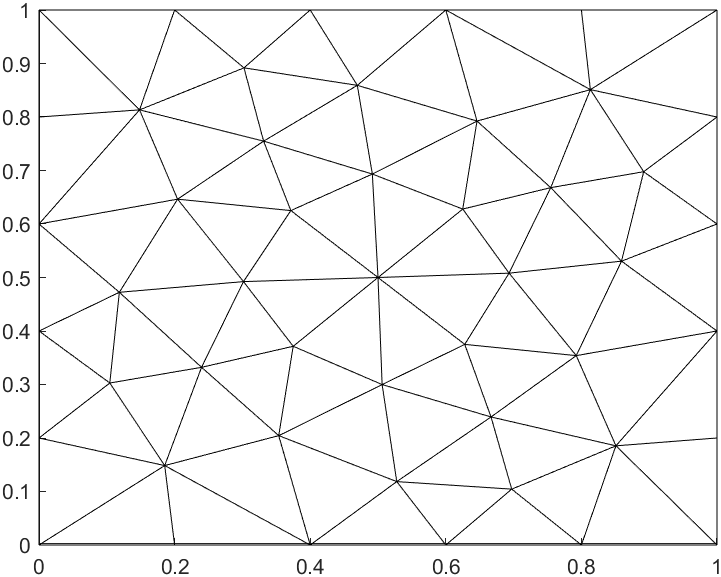
\includegraphics[width=\textwidth]{report/Images/Software/Gmsh meshing algorithms/gmsh_meshing_algorithms_meshadapt.png}
        \end{subfigure}
        \begin{subfigure}[b]{0.33\textwidth}
            \centering
            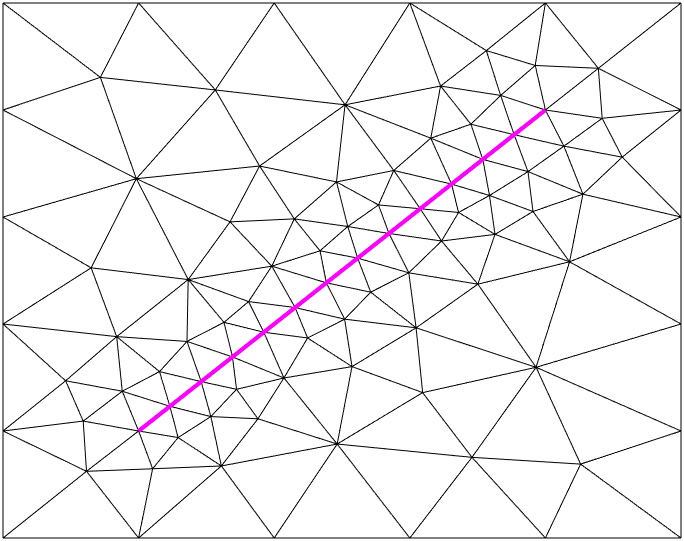
\includegraphics[width=\textwidth]{report/Images/Software/Gmsh meshing algorithms/gmsh_meshing_algorithms_embedded_meshadapt.png}
        \end{subfigure}
        \caption{MeshAdapt}
        \label{fig:Gmsh-MeshAdapt}
    \end{subfigure}
    \begin{subfigure}[b]{\textwidth}
    \centering
        \begin{subfigure}[b]{0.33\textwidth}
            \centering
            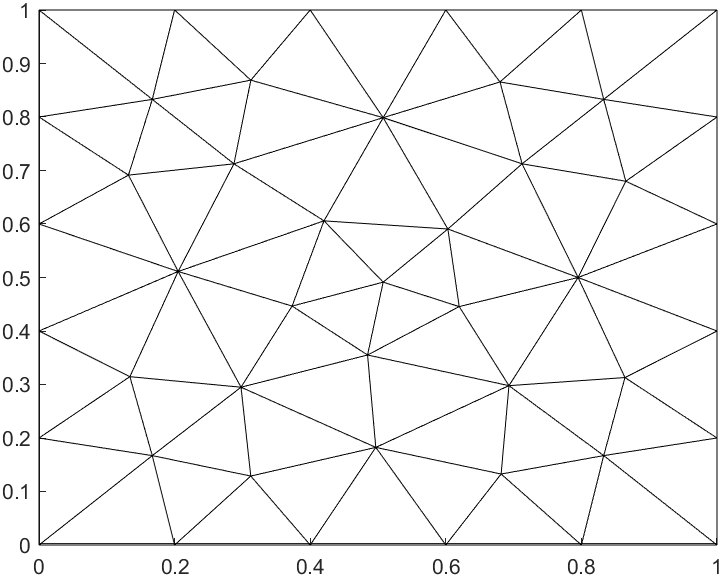
\includegraphics[width=\textwidth]{report/Images/Software/Gmsh meshing algorithms/gmsh_meshing_algorithms_delaunay.png}
        \end{subfigure}
        \begin{subfigure}[b]{0.33\textwidth}
            \centering
            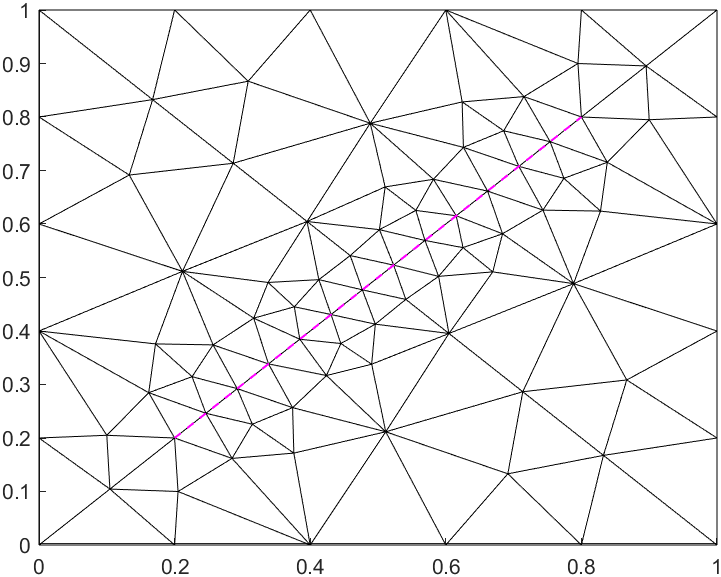
\includegraphics[width=\textwidth]{report/Images/Software/Gmsh meshing algorithms/gmsh_meshing_algorithms_embedded_delaunay.png}
        \end{subfigure}
        \caption{Delaunay}
        \label{fig:Gmsh-Delaunay}
    \end{subfigure}
    \begin{subfigure}[b]{\textwidth}
        \centering
        \begin{subfigure}[b]{0.33\textwidth}
            \centering
            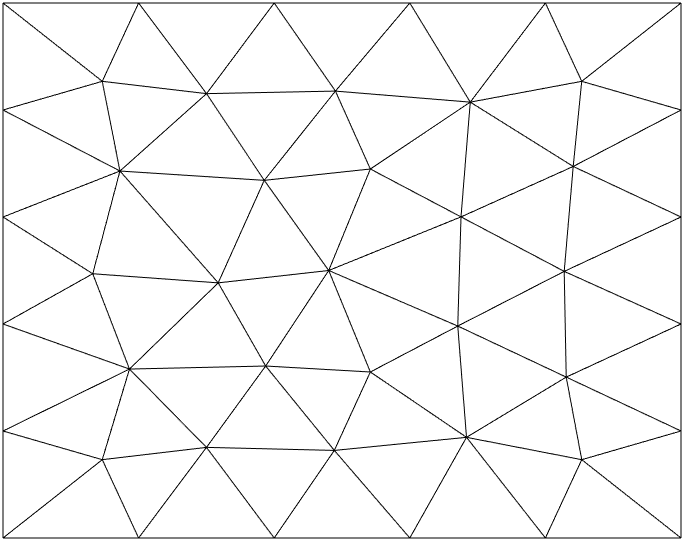
\includegraphics[width=\textwidth]{report/Images/Software/Gmsh meshing algorithms/gmsh_meshing_algorithms_frontal.png}
        \end{subfigure}
        \begin{subfigure}[b]{0.33\textwidth}
            \centering
            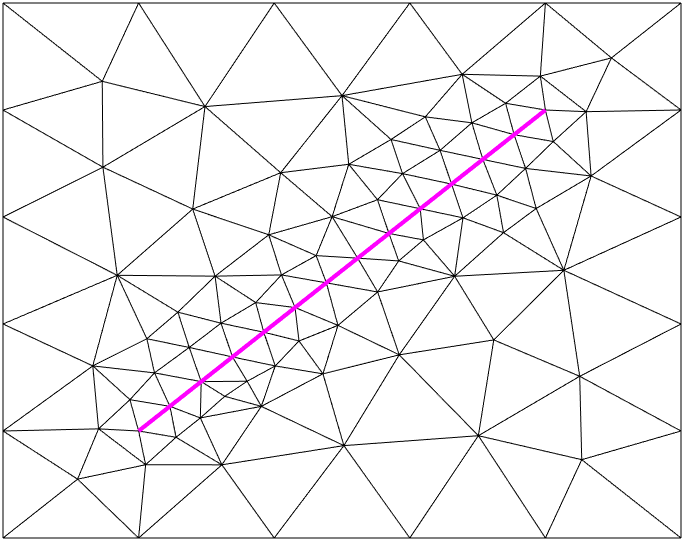
\includegraphics[width=\textwidth]{report/Images/Software/Gmsh meshing algorithms/gmsh_meshing_algorithms_embedded_frontal.png}
        \end{subfigure}
        \caption{Frontal-Delaunay}
        \label{fig:Gmsh-Frontal-Delaunay}
    \end{subfigure}
    \begin{subfigure}[b]{\textwidth}
        \centering
        \begin{subfigure}[b]{0.33\textwidth}
            \centering
            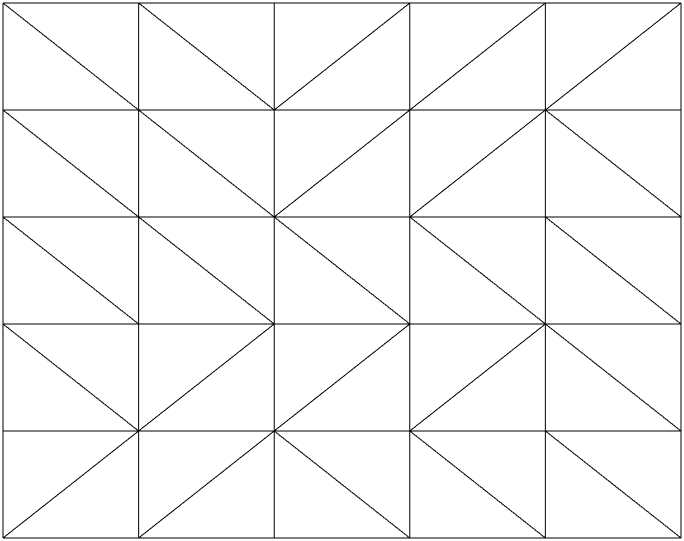
\includegraphics[width=\textwidth]{report/Images/Software/Gmsh meshing algorithms/gmsh_meshing_algorithms_delquad.png}
        \end{subfigure}
        \begin{subfigure}[b]{0.33\textwidth}
            \centering
            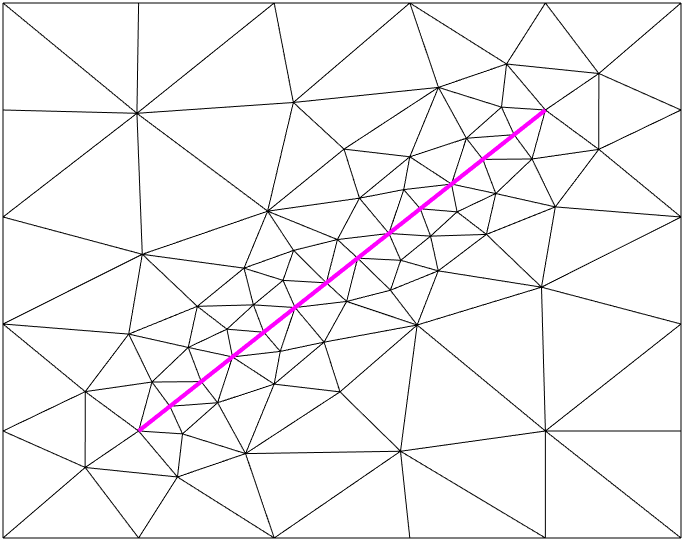
\includegraphics[width=\textwidth]{report/Images/Software/Gmsh meshing algorithms/gmsh_meshing_algorithms_embedded_delquad.png}
        \end{subfigure}
        \caption{Frontal-Delaunay for Quads}
        \label{fig:Gmsh-Frontal-Quads}
    \end{subfigure}
    \begin{subfigure}[b]{\textwidth}
        \centering
        \begin{subfigure}[b]{0.33\textwidth}
            \centering
            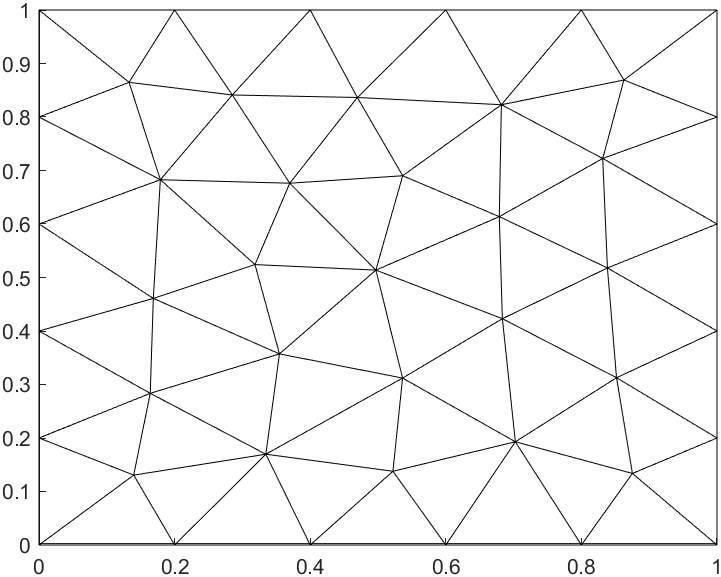
\includegraphics[width=\textwidth]{report/Images/Software/Gmsh meshing algorithms/gmsh_meshing_algorithms_bamg.png}
        \end{subfigure}
        \begin{subfigure}[b]{0.33\textwidth}
            \centering
            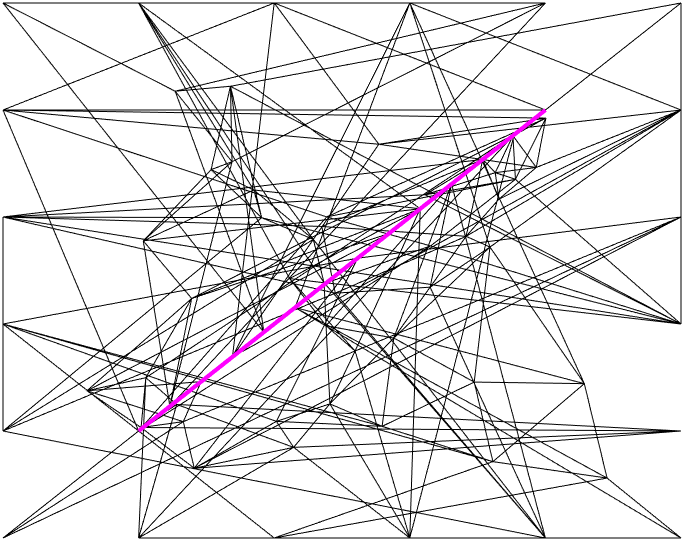
\includegraphics[width=\textwidth]{report/Images/Software/Gmsh meshing algorithms/gmsh_meshing_algorithms_embedded_bamg.png}
        \end{subfigure}
        \caption{BAMG}
        \label{fig:Gmsh-BAMG}
    \end{subfigure}
    \caption[Comparison of the Gmsh meshing algorithms]{Comparison of the Gmsh meshing algorithms. The left set of meshes are empty, while the right set have an embedded face constraint marked in magenta. Note that BAMG fails to create a quality mesh with an embedded line.}
    \label{fig:Gmsh-meshing-algorithms}
\end{figure}

Gmsh is primarily aimed at creating unstructured meshes. It does, however, provide some methods for generating structured meshes, including support for transfinite meshes \cite{Gmsh_article}. While these require some manual work to work nicely, they provide a way to generate structured, controlled meshes. An example of transfinite meshes is shown in \autoref{fig:py:Gmsh-transfinite}, with code in Python \ref{py:Gmshtransfinite}.

\emph{The Solver module} provides two ways to connect Gmsh to external finite element solvers. The most straight-forward way is by directly using the Gmsh API to load geometry, meshes and data \cite{Gmsh_article}. This method requires a significant programming investment from the solver developers, as the connection between the solver and the API must be created.

To maintain the goal of being a user friendly generator, Gmsh provides a Gmsh interface through Unix or TCP/IP sockets \cite{Gmsh_article}. This lets a user launch solvers directly from Gmsh, and requires few adaptations of the solver software. Solvers are outside the scope of this thesis.

\emph{The Post-Processing module} enables loading and display of data views, alongside the geometry and mesh \cite{Gmsh_article}. Views are collections of values - both scalar and tensors, where scalar fields can be visualized as iso-surfaces or color maps and vector fields as arrows or displacement maps. Post-processing is outside the scope of this thesis. 


\subsubsection{Examples}
\label{sec:Gmsh-examples}
While Gmsh is designed to be user friendly, the scope of features and interfaces make the provided APIs somewhat complex. This section will present some basic examples of Gmsh programs, as well as their outputs. Source code for the examples is shown in \autoref{app:Gmsh-examples}.

\paragraph{Simple square mesh}
While a square mesh is simple to envision, the creation of one requires a bit of code. Python \ref{py:Gmshgrid} shows how this can be implemented, using Gmsh's Python API. The output is shown in \autoref{fig:py:Gmsh-grid}.


\begin{figure}[htp]
    \centering
    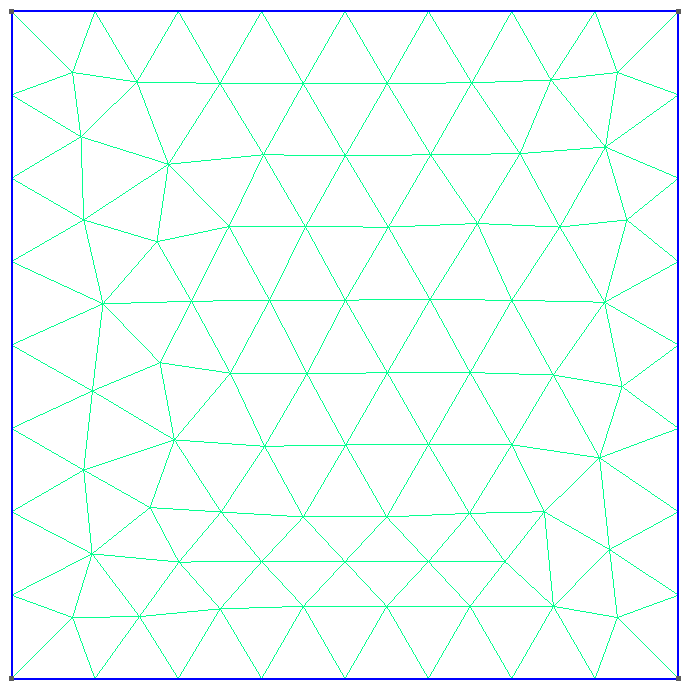
\includegraphics[width=0.6\textwidth]{report/Images/Software/Gmsh examples/gmsh_square_mesh.png}
    \caption[Simple square grid generated in Gmsh]{Simple square grid generated in Gmsh. Output from Python \ref{py:Gmshgrid}.}
    \label{fig:py:Gmsh-grid}
\end{figure}


\paragraph{Adjusting the mesh size field}
Gmsh offers two ways to adjust the produced mesh. The first option, as shown in \autoref{fig:Gmsh-meshing-algorithms}, is to embed lines in the mesh, making Gmsh use the lines as faces in the mesh. The second method is to adjust the mesh size field function.

An example of the latter method is shown in Python \ref{py:Gmshfield}, with output in \autoref{fig:py:Gmsh-field}. In the example, we use a line as basis for a threshold field which scales the mesh size based on distance from the line. We also use a point as basis for a math field which scales the mesh size based on the square of the distance from the point. We finally combine the fields by using the minimum mesh size. Note that neither the point nor the line are embedded in the mesh, meaning that there is no guarantee that the faces of the mesh align with either. The example also shows how Gmsh can connect to multiple CAD kernels - in this case using the OpenCASCADE kernel \cite{Gmsh_reference}.

\begin{figure}[htp]
    \centering
    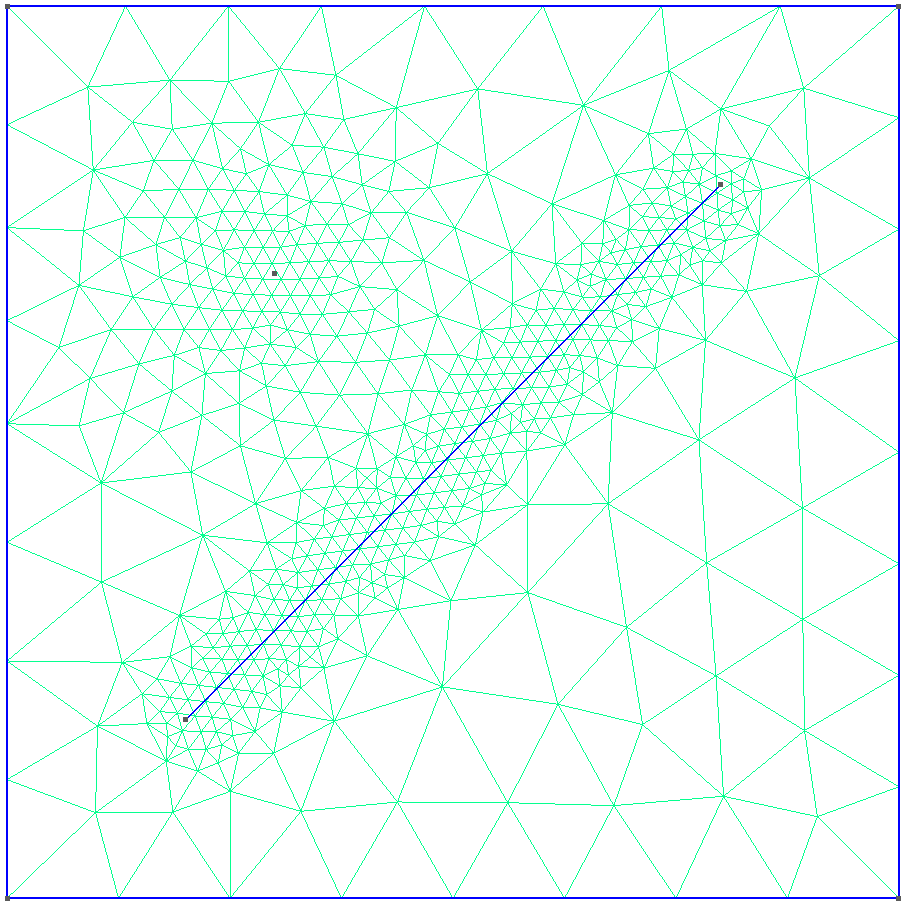
\includegraphics[width=0.6\textwidth]{report/Images/Software/Gmsh examples/gmsh_mesh_size_fields.png}
    \caption[Adjusted mesh size field generated in Gmsh]{Adjusted mesh size field generated in Gmsh. Output from Python \ref{py:Gmshfield}.}
    \label{fig:py:Gmsh-field}
\end{figure}

\paragraph{Structured meshes}
Structured meshes can be created by using transfinite curves and surfaces. An example of this is shown in Python \ref{py:Gmshtransfinite}, with output in \autoref{fig:py:Gmsh-transfinite}. In the example, two transfinite meshes are created. The green mesh consists of linearily distributed transfinite nodes, while the orange consists of nodes following a geometric progression with power $1.5$. The cyan mesh is a standard unstructured mesh. To get rectangular cells, we use the recombine feature, combining the triangular grid into quadrilaterals within the transfinite meshes.

\begin{figure}[htp]
    \centering
    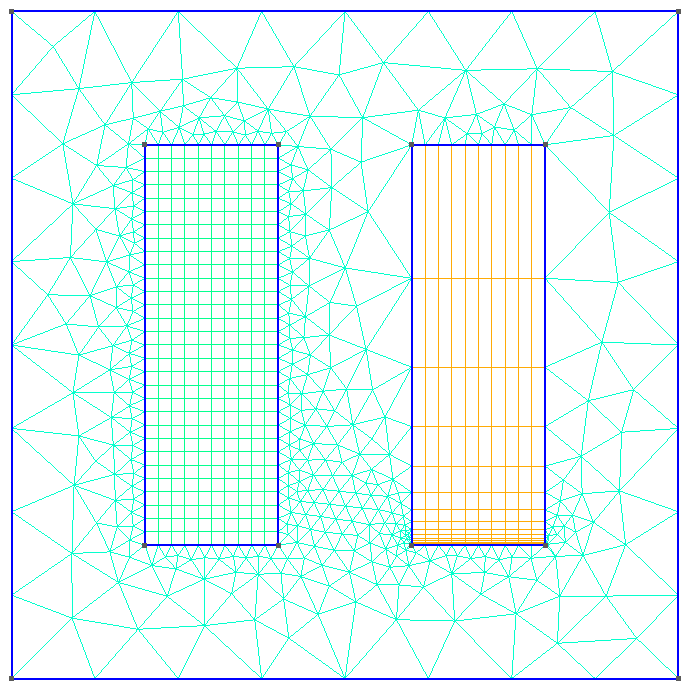
\includegraphics[width=0.7\textwidth]{report/Images/Software/Gmsh examples/gmsh_structured_meshes.png}
    \caption[Structured meshes generated in Gmsh]{Structured meshes generated in Gmsh. Output from Python \ref{py:Gmshtransfinite}.}
    \label{fig:py:Gmsh-transfinite}
\end{figure}

\subsubsection{Limitations}
Although Gmsh is a well-developed solution for both meshing and CAD work, it does have some limitations - especially when combining it with MRST and UPR. One key difference between the two systems arise from the fact that Gmsh operates with triangulations, while MRST operates with PEBI grids. As these are dualities, we can easily convert between triangulation nodes to PEBI sites. This does, however, have a potential of losing information about cell faces.

When converting from a triangulation to a PEBI grid, vertices in the triangulation are used as sites in the PEBI grid, and two sites connected in the triangulation share a PEBI face. As such, any face constraint in the triangulation is guaranteed to have a cell path in the PEBI grid, but there is no guarantee for the width of the path. This is especially true when the path is turning. An even bigger issue arises from cell constraints in the triangulation. There is no guarantee of triangulation cell centers ending up on a PEBI face, and even less chance of the faces aligning with the cell constraints.

An illustration of this challenge is shown in \autoref{fig:triangulation-to-PEBI-limitation}. The cells of the PEBI grid align somewhat nicely with the cell constraint on straight lines, but fails without detailed manual control in the corners. The vertices of the PEBI grid are somewhat close to the face constraint, but the edges do not align with the constraint line.

\begin{figure}[ht]
    \centering
    \begin{subfigure}[b]{0.45\textwidth}
        \centering
        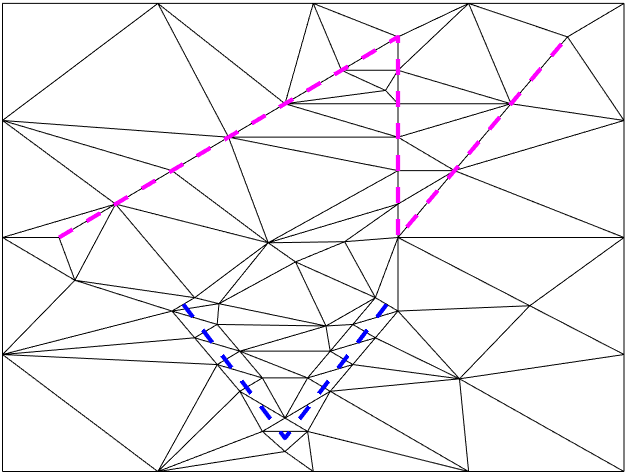
\includegraphics[width=\textwidth]{report/Images/Software/Gmsh limitations/gmsh_conversion_triangulation.png}
        \caption{Triangulation}
        \label{fig:limitation-triangulation}
    \end{subfigure}
    \begin{subfigure}[b]{0.45\textwidth}
        \centering
        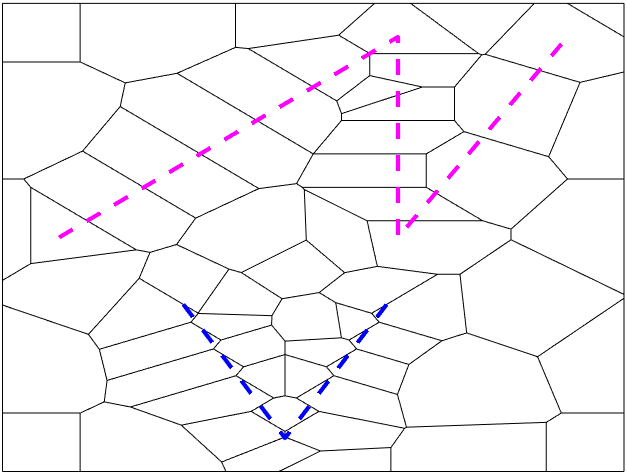
\includegraphics[width=\textwidth]{report/Images/Software/Gmsh limitations/gmsh_conversion_PEBI.png}
        \caption{PEBI grid}
        \label{fig:limitation-pebi}
    \end{subfigure}
    \caption[Misaligned constraints when converting triangulation to PEBI grid]{Illustration of misaligned constraints when converting a triangulation to a PEBI grid. The magenta line represents a face constraint in the triangulation, and should preferably be a cell constraint in the PEBI grid. The blue line represents a cell constraint in the triangulation, and should preferably be a face constraint in the PEBI grid.}
    \label{fig:triangulation-to-PEBI-limitation}
\end{figure}

% No way to manually adjust mesh - must use fields

